\section{User Guide}\label{user-guide}

This chapter walks through KompozeR from the point of view of its three
roles:\texttt{GUEST}, \texttt{BASE} and \texttt{ADMIN} following the navigation structure of the
frontend. The interface itself is in Italian (for now).

\subsection{Access}\label{ug-access}

KompozeR is reached at the frontend's URL (\cref{deployment}), which shows a
single card with two tabs, ``Accedi'' (Log in) and ``Registrati'' (Register),
plus a divider and a ``Continua come ospite'' (Continue as guest) button.

\begin{figure}[h!]
\centering
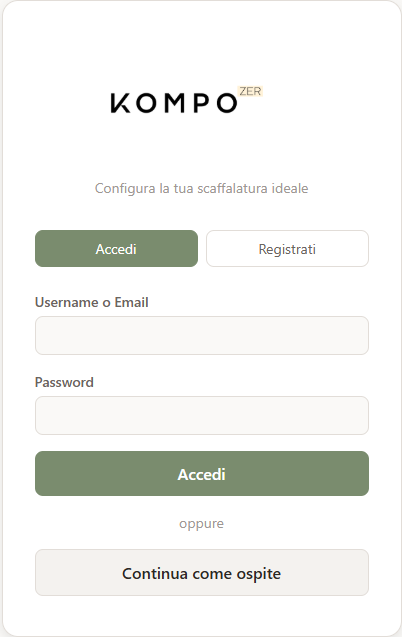
\includegraphics[width=0.4\linewidth]{images/1.png}
\caption{AuthView: card login/registration with Guest button.}
\label{fig:auth-view}
\end{figure}

\begin{itemize}
  \item \textbf{Registering} asks for Username, Nome (first name), Cognome
  (last name), Email and Password (minimum 8 characters); on success the new
  user is shown a confirmation dialog and returned to the login tab with
  their identifier pre-filled.

  \item \textbf{Logging in} accepts either the username or the email plus
  the password. A wrong password or an unknown identifier produce a clear
  inline error (``Password Errata'' / ``Utente Non Trovato'').

  \item \textbf{Continuing as guest} skips registration entirely and opens a
  temporary \texttt{GUEST} session (FR1), useful for trying the configurator
  without commitment; a guest cannot save a configuration under a profile
  (FR6) or reach the catalog/admin screens.
\end{itemize}

Once logged in, a header bar appears at the top of every screen with
navigation links (varying by role), a cart icon, a
notification bell for authenticated non-guest users, the current
username (or ``Guest''), and an ``Esci'' (Log out) button.

\begin{figure}[h!]
\centering

\includegraphics[width=0.4\linewidth]{images/2.png}
\caption{AppHeader: Navigation ber for BASE user.}
\label{fig:app-header}
\end{figure}


\subsection{Building a configuration}\label{ug-configurator}

The configurator (route \texttt{/cad}) is the core of the product (FR1) and
is organised as a five-step wizard, matching the \texttt{Configuration}
lifecycle of \cref{behaviour}: ``Ambiente'' (environment),
``Categoria'' (product family), ``Colonne'' (columns), ``Design'' and
``Finalizza'' (finalise). A BOM panel and a live schematic are always
visible on the side, updated after every step.

\begin{figure}[h!]
\centering
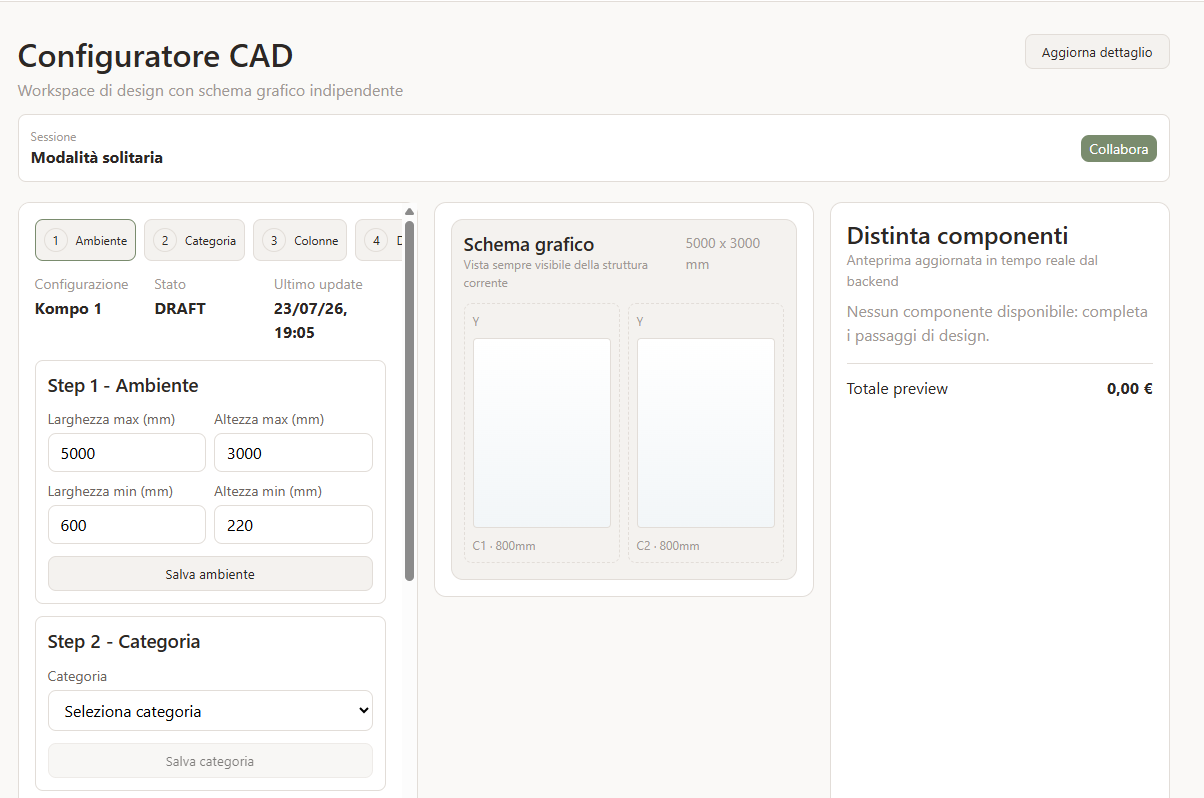
\includegraphics[width=0.4\linewidth]{images/3.1.png}
\caption{CadView: the five-step wizard with the BOM/preview panel.}
\label{fig:cad-view}
\end{figure}


\begin{enumerate}
  \item \textbf{Starting a configuration.} From ``Configurazioni'' (or
  directly from the configurator), enter a name, optionally pick a starting
  product family, and press ``Crea e apri in CAD'' (Create and open in CAD).

  \item \textbf{Ambiente.} Enter the minimum and maximum width/height (mm)
  the finished unit must fit, then ``Salva ambiente'' (FR1).

  \item \textbf{Categoria.} Choose one of the four mutually incompatible
  product families:Tondo, Quadro, Kube, Intelligente then ``Salva categoria''. Changing this later
  discards any column plan or design already produced, with a two-step
  confirmation dialog.

  \item \textbf{Colonne.} Choose how many columns (1--8) and a width for
  each, picked from the widths actually available for the selected family,
  then ``Salva piano colonne'' (FR9: only compatible widths are offered, so
  an invalid combination cannot be composed in the first place).

  \item \textbf{Design.} For each column, add or remove shelf levels one at
  a time (``+ Livello'' / ``- Ultimo''); only heights that keep the design
  physically valid are offered, and an explanatory reason is shown when a
  candidate height is unavailable (e.g.\ too close to another shelf, or
  exceeding the maximum height). For the Intelligente family, adding a level
  applies it to every column at once, automatically distinguishing outer
  columns (``BORDO'') from inner ones (``INTERMEZZO''). The BOM panel and
  price update after every change (FR2, FR3).
  \begin{figure}[h!]
  \centering
  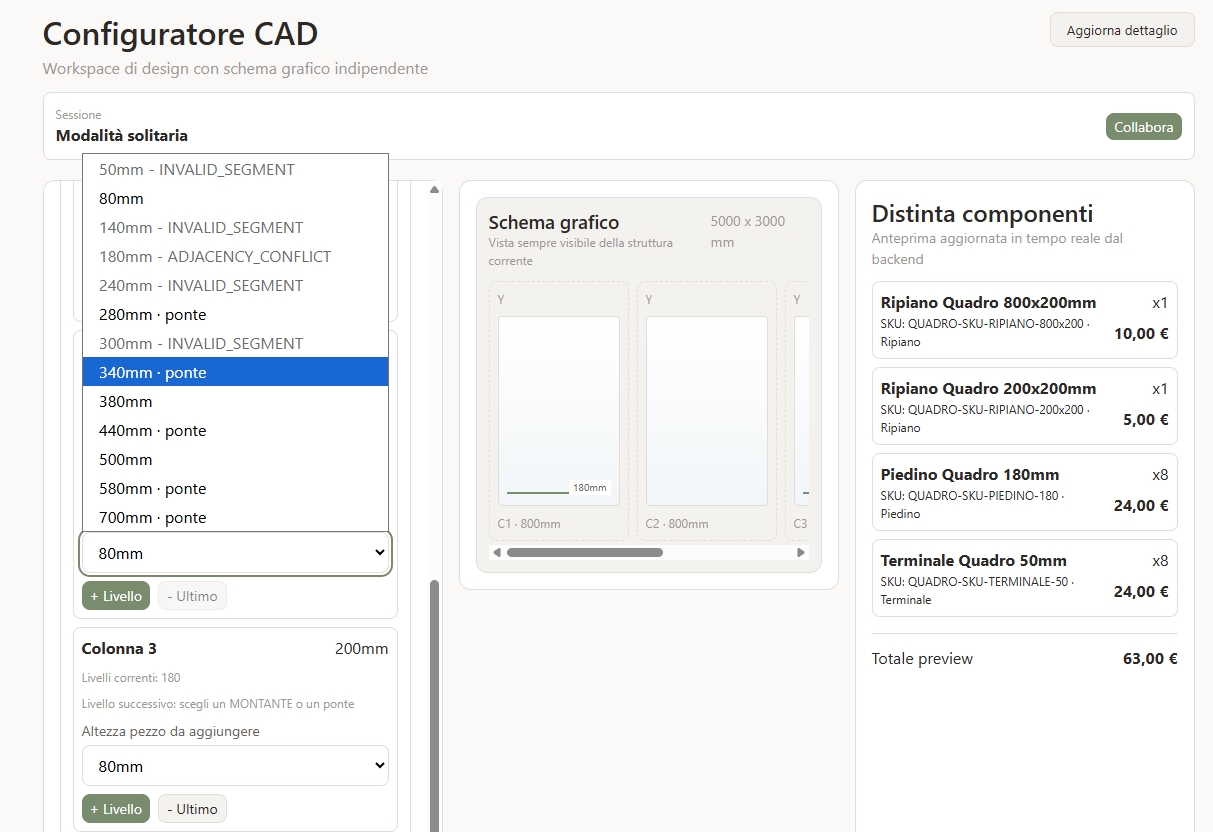
\includegraphics[width=0.4\linewidth]{images/4.png}
  \caption{CadView step 4: level-by-level design with the reason codes.}
  \label{fig:cad-view}
  \end{figure}


  \item \textbf{Finalizza.} Once the design is complete, ``Finalizza e invia
  al carrello'' (Finalise and send to cart) is enabled, moving the
  configuration to its terminal \texttt{FINALIZED} state and adding its BOM
  to the cart in one action (FR4).
\end{enumerate}

\subsection{Collaborating on a configuration}\label{ug-collab}

While editing, the owner can press ``Collabora'' to open a collaborative
session: a short, unambiguous code is shown in a dialog with a ``Copia codice'' (copy) button.

\begin{figure}[h!]
\centering
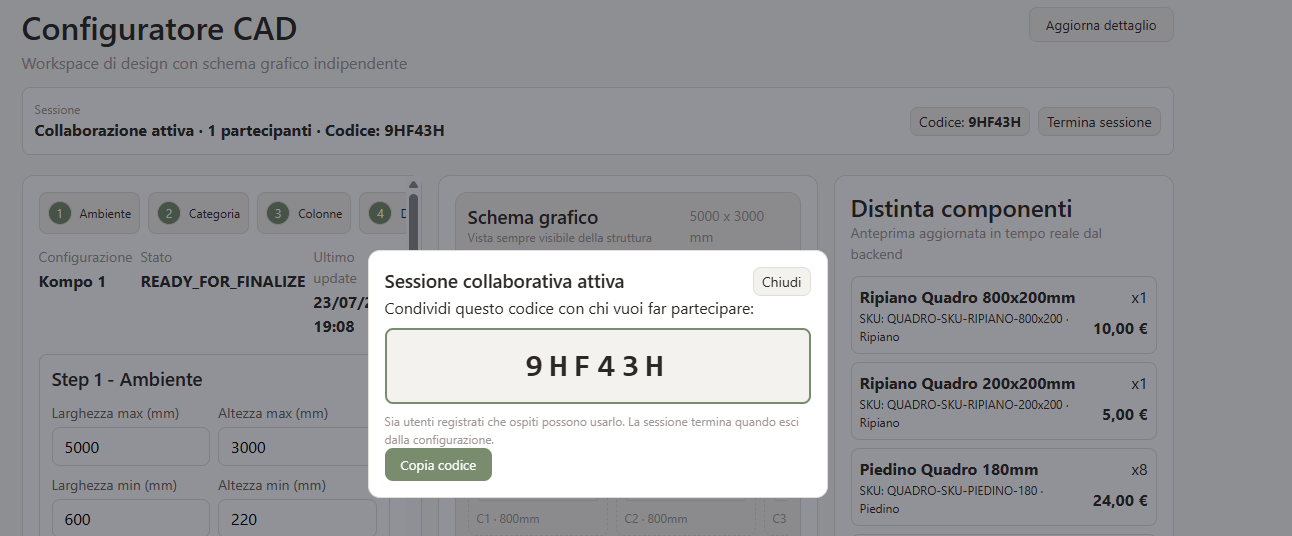
\includegraphics[width=0.4\linewidth]{images/5.png}
\caption{CadView: the "Sessione collaborativa attiva" dialog with the session code.}
\label{fig:cad-view}
\end{figure}

Another user opens the same configuration's join box, types the code
(``Entra con codice''), and immediately sees the same environment, category,
column plan and design as the owner; from then on, edits from either
participant appear on the other's screen in real time, resolved
deterministically if both edit the same field at once. 
A status line (``Collaborazione attiva ·
$N$ partecipanti'') always shows who is connected; if the owner leaves, the
session ends for everyone with an explicit notice, since the configuration
itself only ever lives in the owner's account.

\begin{figure}[h!]
\centering
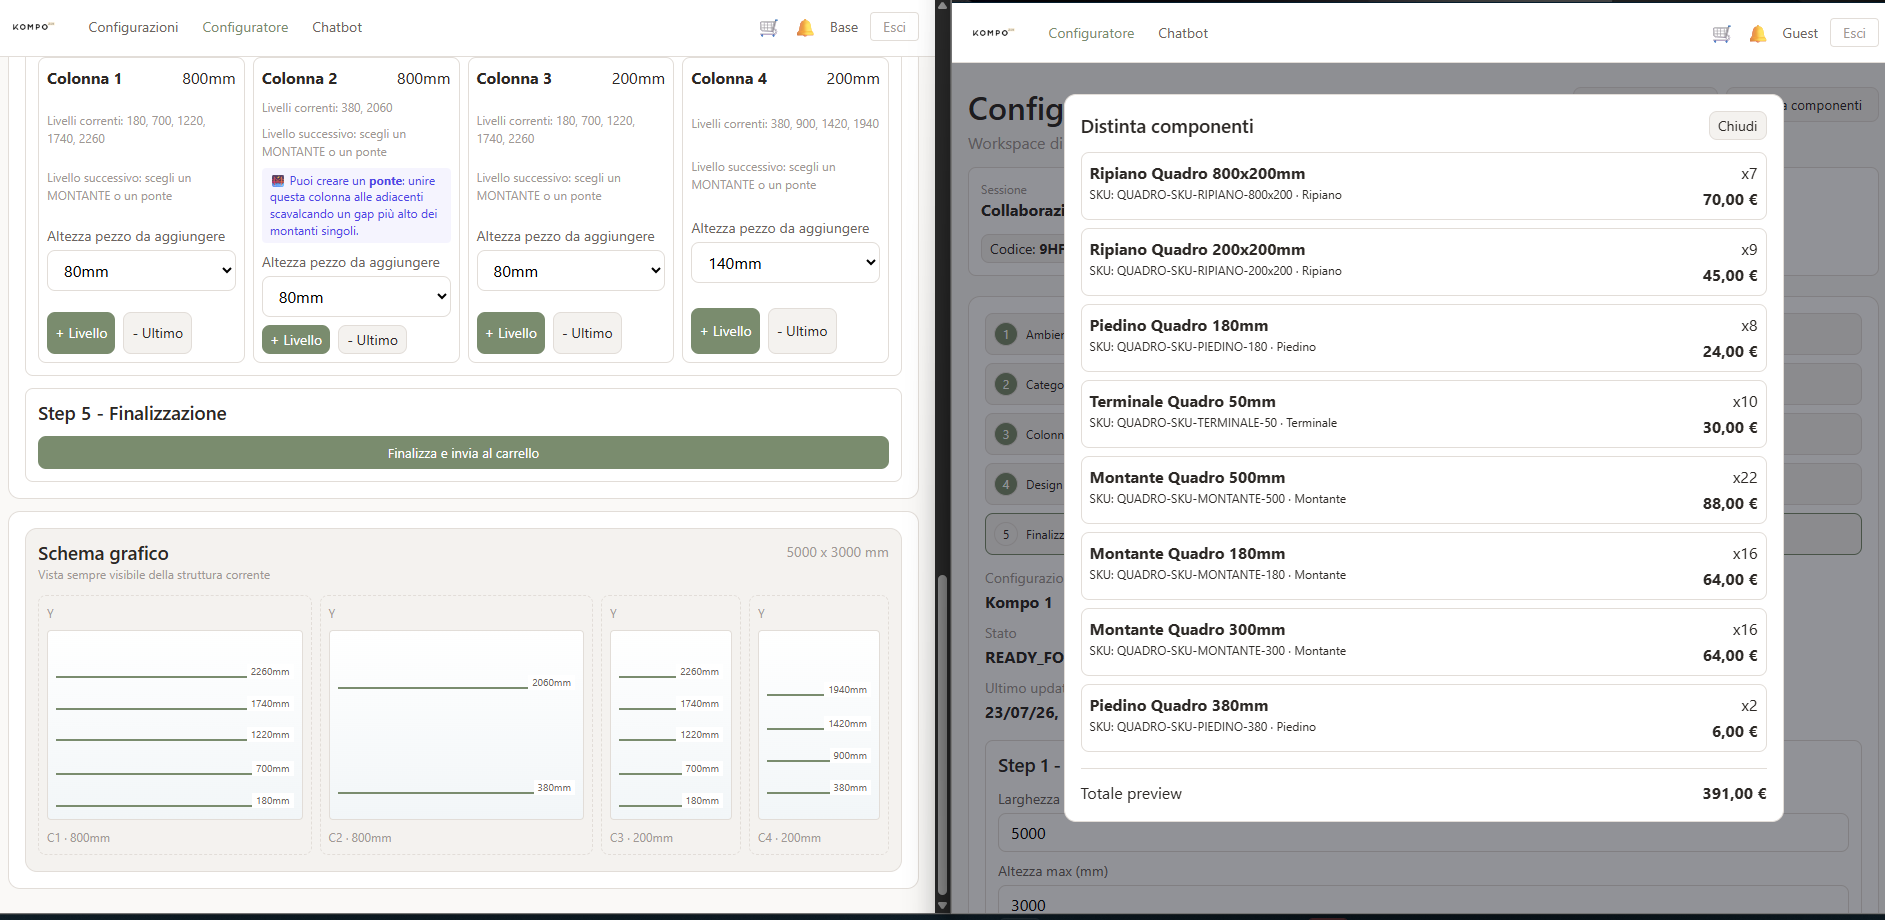
\includegraphics[width=0.4\linewidth]{images/6.1.png}
\caption{CadView: two browser windows showing the same configuration in sync.}
\label{fig:cad-view}
\end{figure}

\subsection{Saving and resuming configurations}\label{ug-saved}

The ``Configurazioni'' screen (route \texttt{/configurations}, \texttt{BASE}
and \texttt{ADMIN} only) lists a logged-in user's own configurations with
summary counters (total, drafts, ready to finalise, finalised, in progress)
and, an ``Apri in CAD'' button to resume
editing (FR6, FR7) and, once \texttt{FINALIZED}, a ``Riordina'' (reorder)
button that adds its BOM straight to the cart again.

\begin{figure}[h!]
\centering
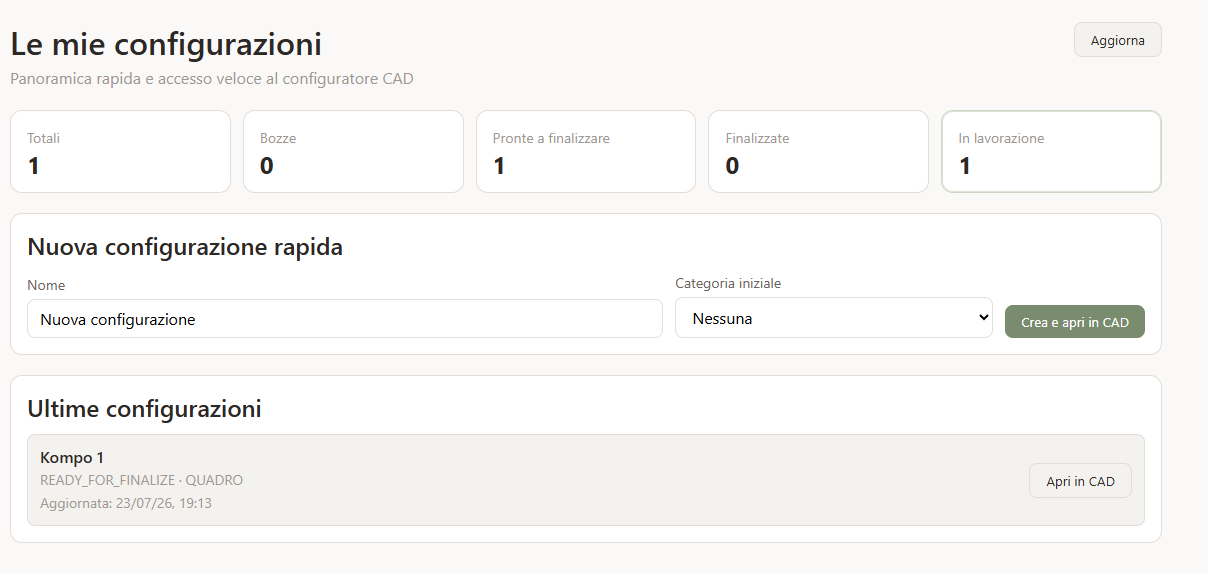
\includegraphics[width=0.4\linewidth]{images/7.png}
\caption{ConfigurationsView: the list of saved configurations with KPI cards.}
\label{fig:configuration-view}
\end{figure}

\subsection{Cart and checkout}\label{ug-cart}

The cart (route \texttt{/cart}) lists every line item with its quantity
(adjustable with +/- buttons) and running total, plus a ``Svuota carrello''
(empty cart) and a ``Procedi al checkout'' button (FR4). If a component in
the cart becomes unavailable in the meantime, it is automatically removed
and the user is told so, rather than being allowed to order something the
catalog can no longer provide.

\begin{figure}[h!]
\centering
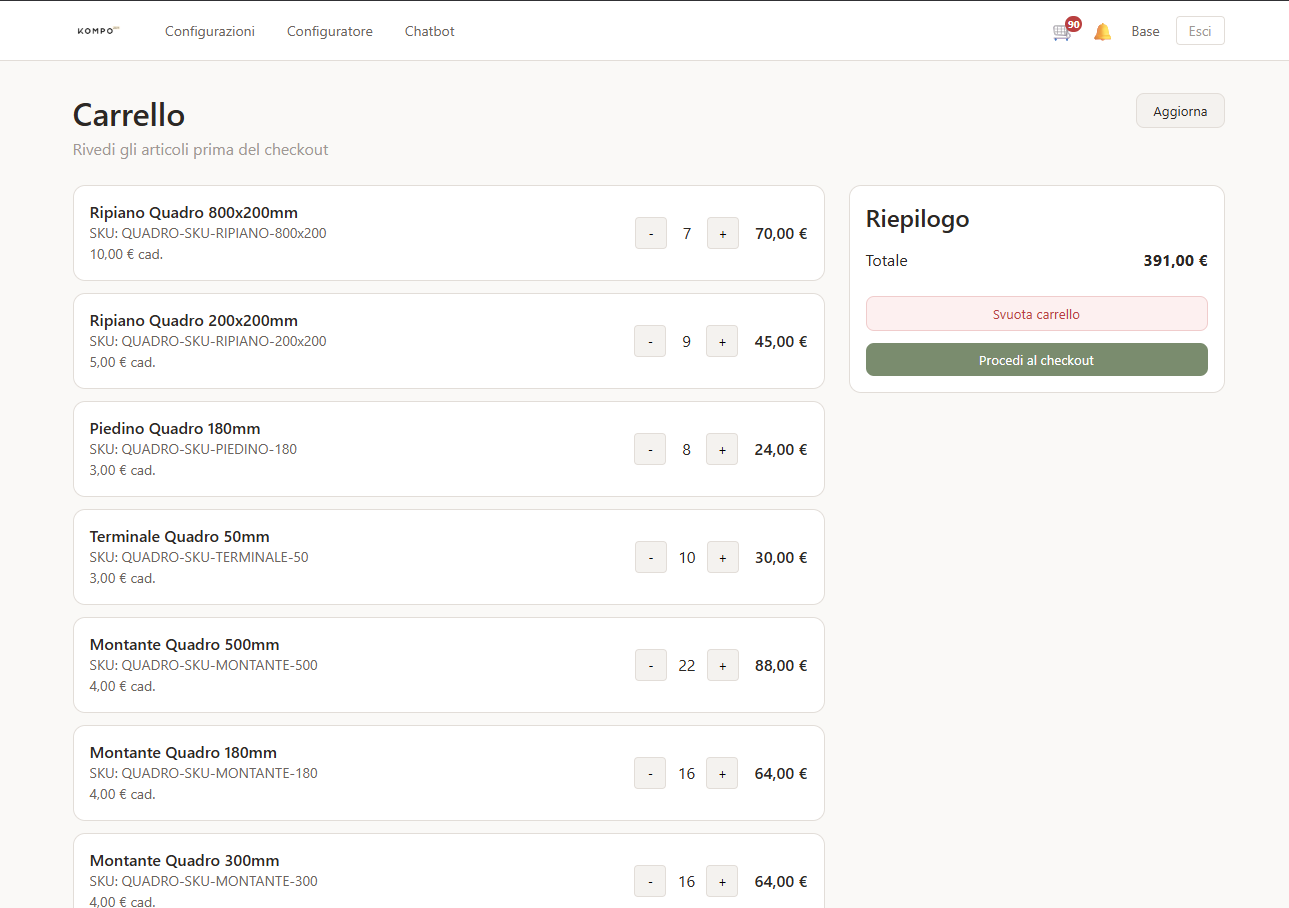
\includegraphics[width=0.4\linewidth]{images/8.png}
\caption{CartView: line items and the checkout summary panel}
\label{fig:cart-view}
\end{figure}

Checkout opens a ``Dati spedizione'' (shipping details) form: name,
surname, email, country, city, postal code, address, phone, and an optional
delivery note. Validated client-side before ``Conferma checkout''
finalises the order.

\begin{figure}[h!]
\centering
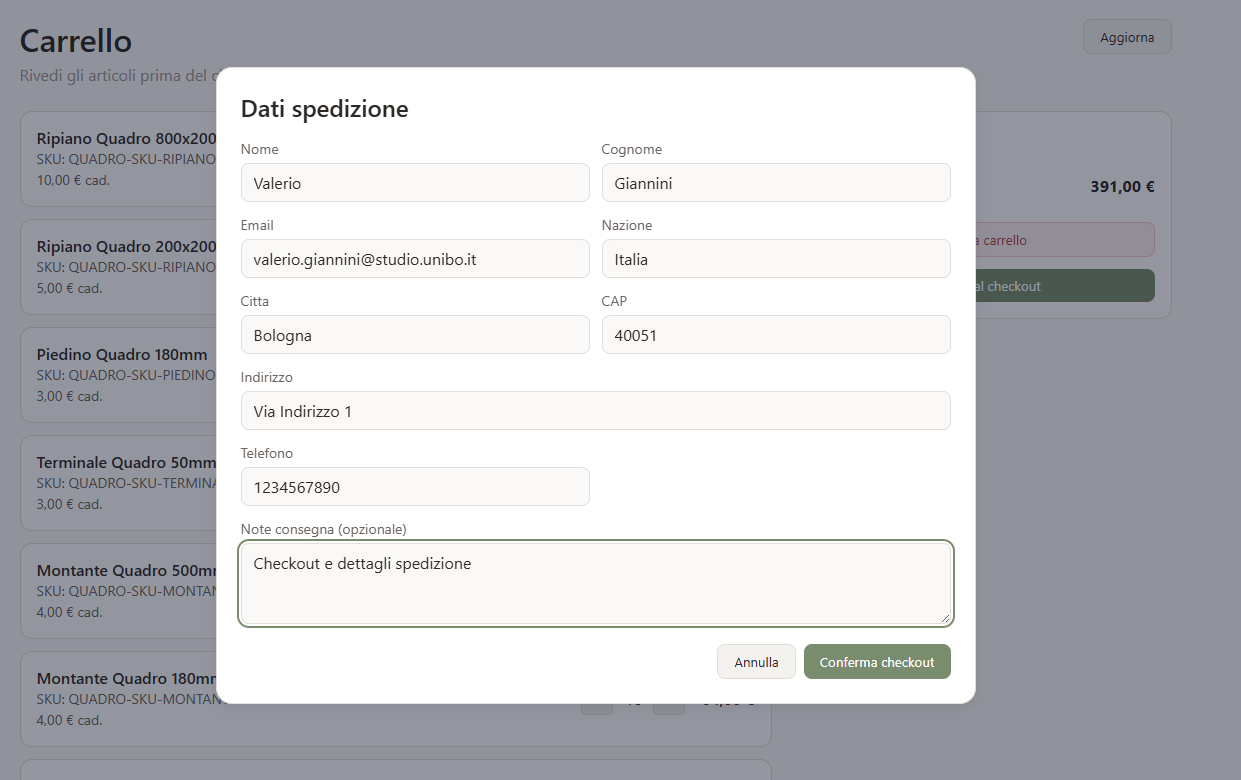
\includegraphics[width=0.4\linewidth]{images/9.png}
\caption{CartView: the shipping-details checkout modal.}
\label{fig:cart-view}
\end{figure}

\subsection{Notifications}\label{ug-notifications}

Authenticated users see a bell icon with an unread-count badge in
the header, updated both by polling and in real time as changes happen
(NFR2). The ``Notifiche'' screen lists every notification (a price or
availability change affecting a subscribed component, FR8) with a filter for
unread-only and a button to mark one as read.

\begin{figure}[h!]
\centering
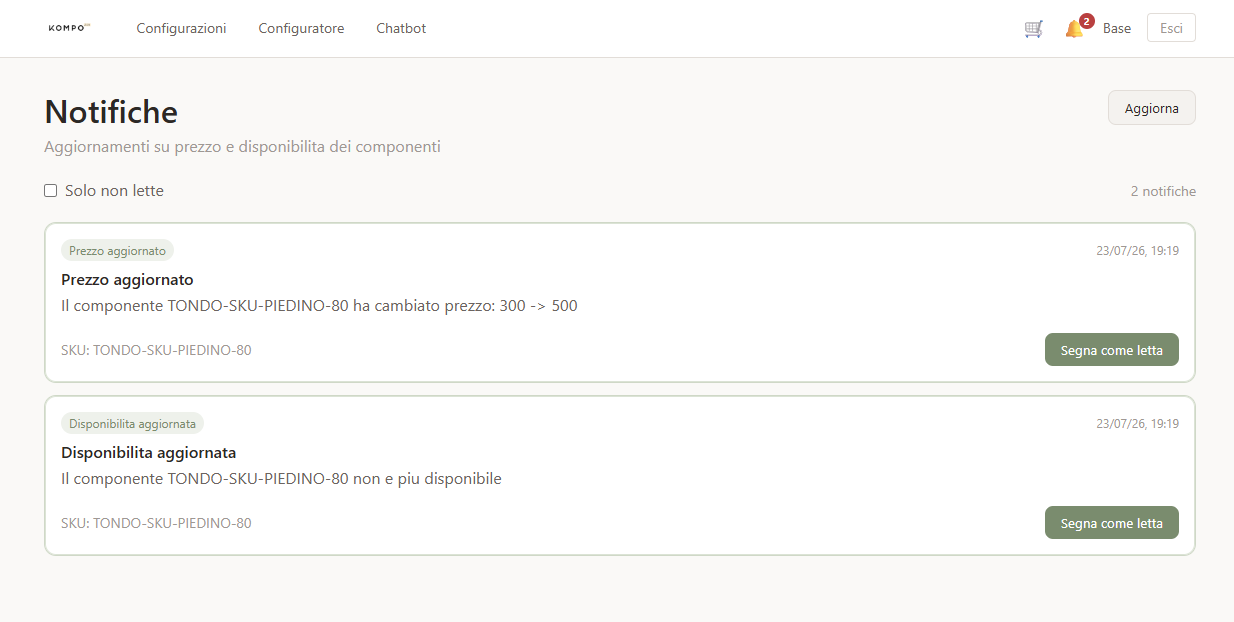
\includegraphics[width=0.4\linewidth]{images/10.png}
\caption{NotificationsView — the notification list.}
\label{fig:notification-view}
\end{figure}

\subsection{Chatbot}\label{ug-chatbot}

The chatbot (route \texttt{/chatbot}) is a dedicated chat screen (FR5).
Messages are exchanged like in a normal mesasging app;
a typing indicator shows while the bot is composing an answer, which
can concern, for instance, the current price of a specific component by SKU.

\begin{figure}[h!]
\centering
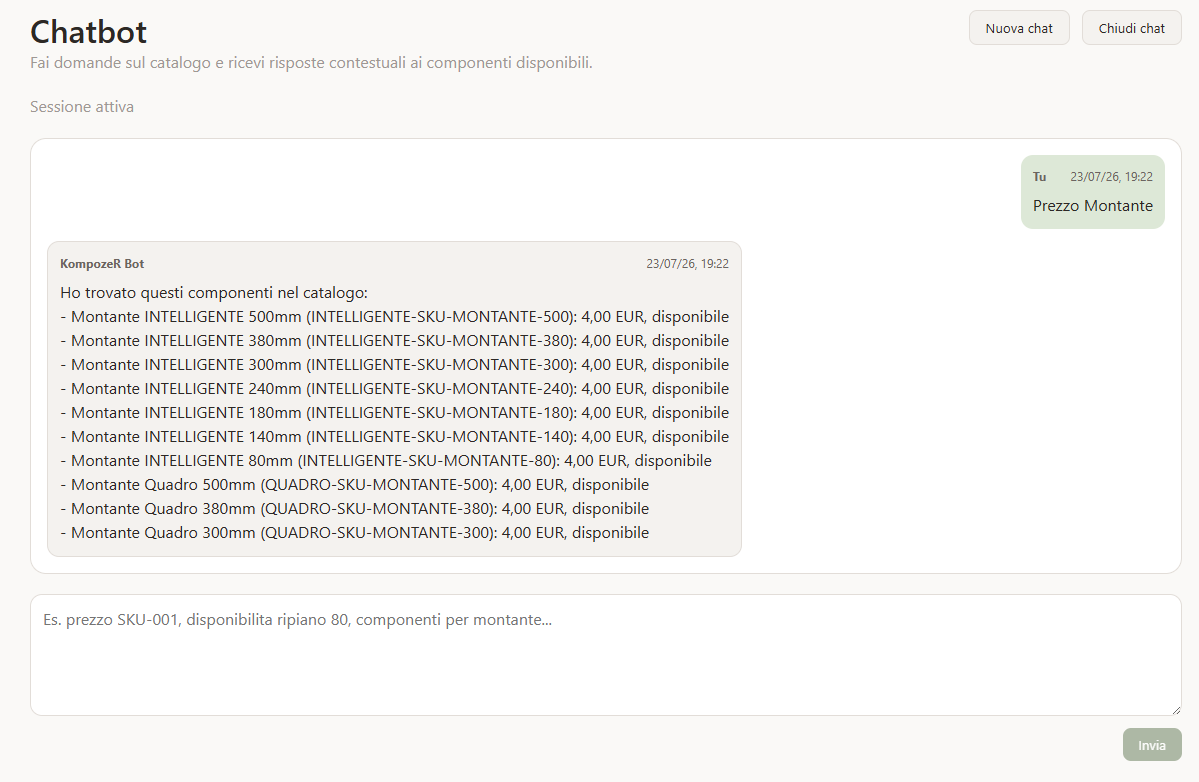
\includegraphics[width=0.4\linewidth]{images/11.png}
\caption{ChatbotView: example of a conversation.}
\label{fig:chatbot-view}
\end{figure}

\subsection{Administration}\label{ug-admin}

\texttt{ADMIN} users additionally see three screens (FR10, FR11), hidden
from every other role (\cref{ug-roles}).

\begin{itemize}
  \item \textbf{``Catalogo Admin''} (route \texttt{/admin/catalog}): add a
  new component (SKU, name, category, type, price, availability,
  description, dimensions, image, compatible category) through a modal
  form, or edit the price/availability of an existing one inline; both
  actions immediately trigger the catalog-change propagation.
  

  \begin{figure}[h!]
  \centering
  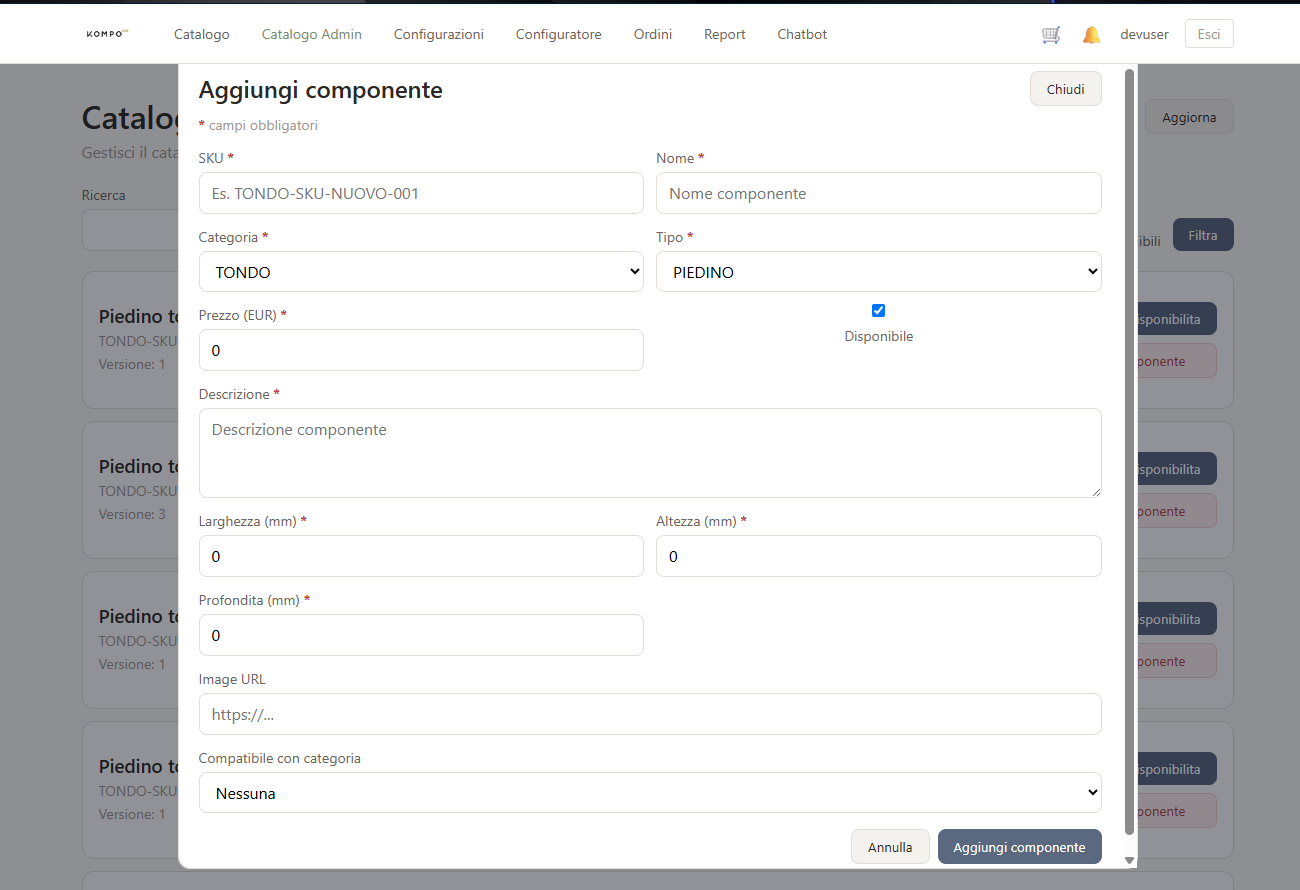
\includegraphics[width=0.4\linewidth]{images/12.1.png}
  \caption{AdminCatalogView: the component list and the "add component" modal.}
  \label{fig:admin-catalog-view}
  \end{figure}

  \item \textbf{``Gestione ordini''} (route \texttt{/admin/orders}): every
  order in the system, filterable by status, with actions to mark a
  \texttt{SUBMITTED} order as ``DONE'' or ``CANCELLED'' (guarded so a
  non-\texttt{SUBMITTED} order cannot be changed twice).

  \begin{figure}[h!]
  \centering
  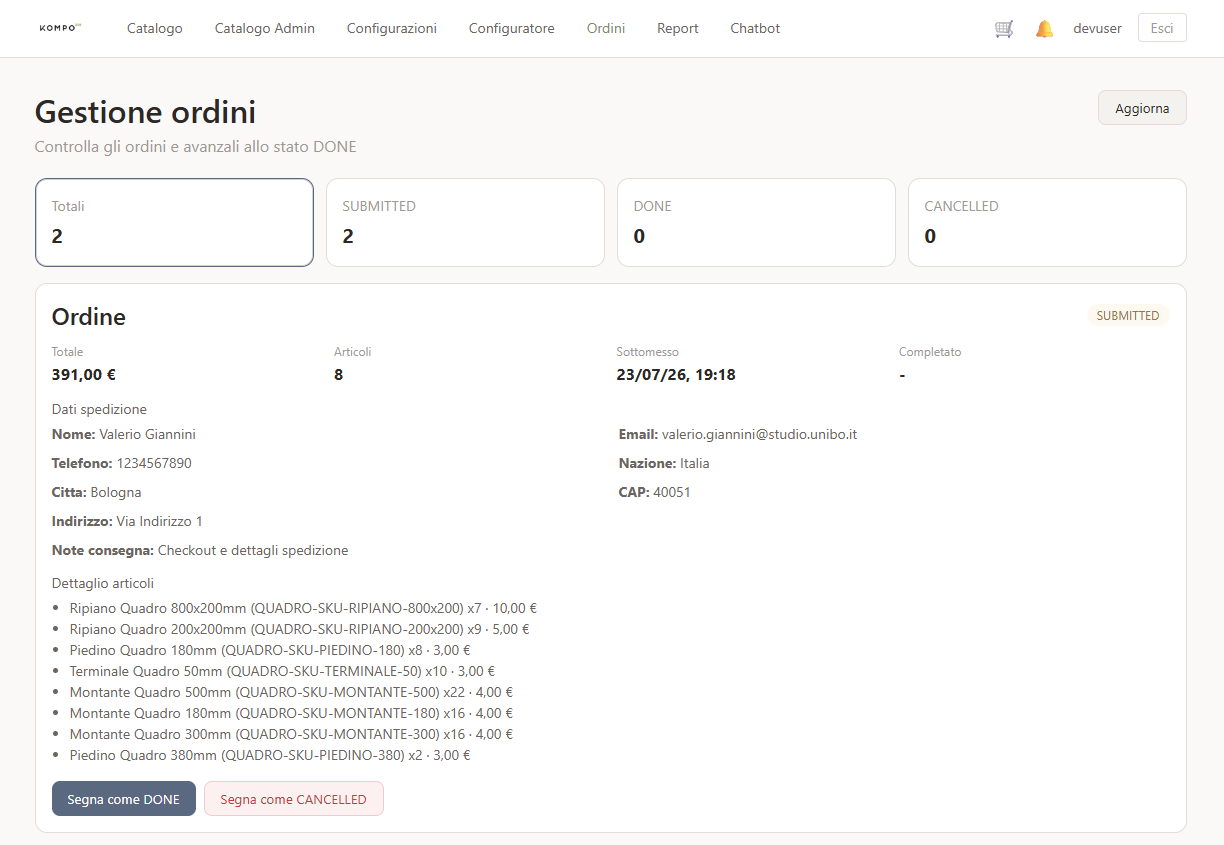
\includegraphics[width=0.4\linewidth]{images/13.png}
  \caption{AdminOrdersView: the order list with status filters.}
  \label{fig:order-view}
  \end{figure}

  \item \textbf{``Report ordini''} (route \texttt{/admin/reports}): a
  date-ranged sales dashboard (total orders, revenue, a per-day breakdown by
  status) computed with a MongoDB aggregation over the order history.

  \begin{figure}[h!]
  \centering
  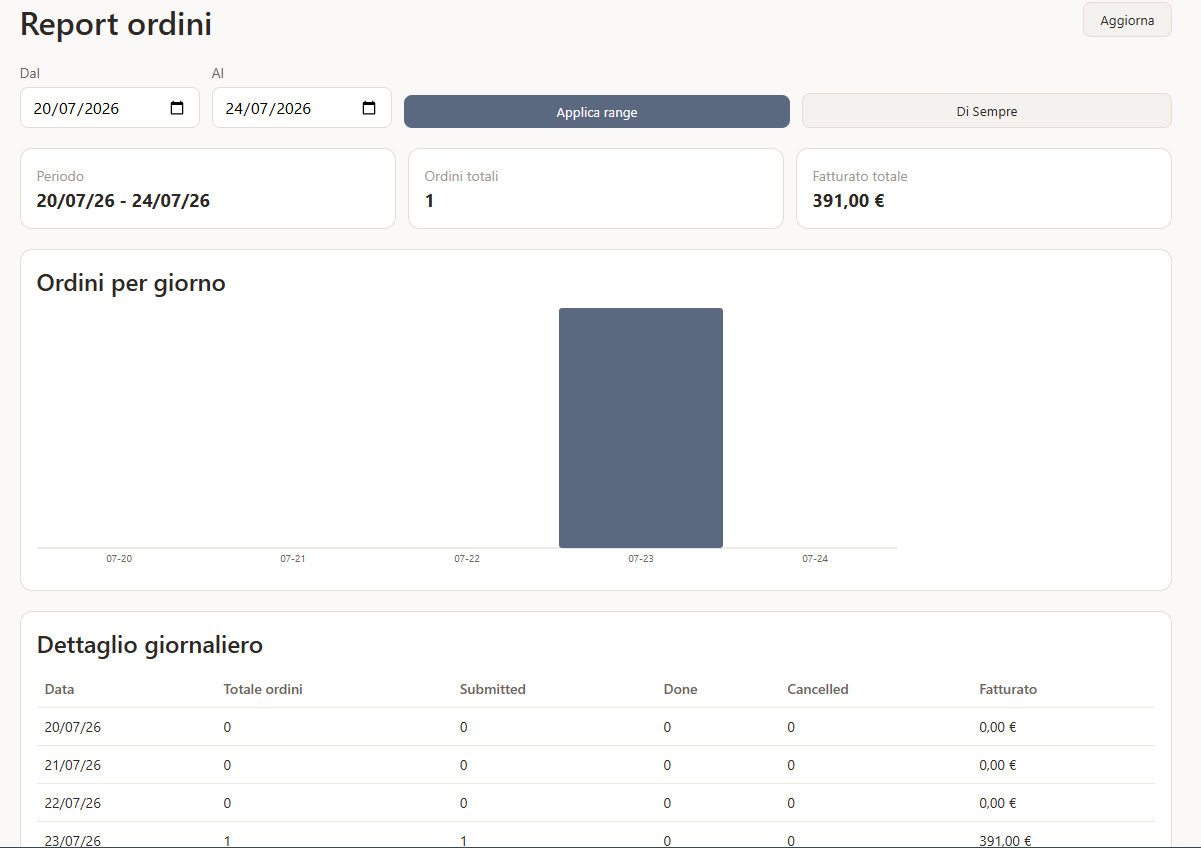
\includegraphics[width=0.4\linewidth]{images/14.png}
  \caption{AdminReportsView: the KPI cards and the per-day chart.}
  \label{fig:report-view}
  \end{figure}
\end{itemize}

\subsection{What each role can see}\label{ug-roles}

The header's navigation links and the router's own guards
(\cref{technological-details}) enforce the same restriction consistently:

\begin{description}
  \item[\texttt{GUEST}] Configuratore, Chatbot only; no saved
  configurations, no cart history beyond the current session, no catalog
  browsing or admin screens.
  \item[\texttt{BASE}] Configurazioni, Configuratore, Chatbot, plus cart and
  notifications; everything a registered customer needs, nothing
  administrative.
  \item[\texttt{ADMIN}] every screen above, plus Catalogo, Catalogo Admin,
  Gestione ordini and Report; an admin's default landing screen is
  ``Gestione ordini'' rather than the configurator.
\end{description}
